% !TEX root = ../main.tex

% ---------------------------------------------------------------
% Background
% ---------------------------------------------------------------

\chapter{Conoscenze Preliminari}\label{chap3:background}
\section{Freezing Of Gait}
È stato dimostrato che il fenomeno del Freezing nella malattia di Parkinson è spesso collegato alle frequenti cadute a cui i soggetti malati vanno incontro. Le cadute nel Parkinson si verificano più spesso quando il soggetto si gira o cambia direzione e sono frequentemente legate a diversi episodi di Freezing. Non tutti i malati di Parkinson subiscono il fenomeno del Freezing, ma si pensa che coloro che lo provano abbiano una più alta probabilità di cadere a terra. L’imprevedibilità del Freezing, accompagnata dallo sforzo inutile a cui il soggetto si sottopone per cercare di muoversi in avanti, possono causare perdita di equilibrio e quindi cadute. \\
Nel tentativo di superare questo stato di forzata immobilità, i pazienti, talora con un aiuto esterno, cercano di mettere in atto adeguate strategie che si avvalgono di stimoli sensoriali di diversa natura (tattili, visivi oppure uditivi e verbali). Alcune tecniche di tipo motorio o sensoriale possono aiutare i pazienti a convivere con il problema del Freezing. Ad esempio, un paziente incapace di iniziare il primo passo potrebbe riuscire a superare il blocco motorio adottando una delle seguenti strategie:
\begin{itemize}
	\item fare un passo in direzione di un bersaglio;
	\item fare un passo per superare un bastone posto sul pavimento;
	\item fare il primo passo marciando come un soldato.
\end{itemize}
L’idea che sta alla base di tali stratagemmi è mettere in atto un programma motorio volontario che sostituisca il programma motorio automatico malfunzionante nei malati di malattia di Parkinson. Episodi frequenti di Freezing possono avere pericolose conseguenze sia sullo stato fisico sia su quello psicologico del malato e compromettono ampiamente la qualità della vita di chi ne soffre privandolo spesso dalla propria indipendenza.\\
\subsection{Le tipologie di Fog}
Il FoG è un episodio transitorio che usualmente dura pochi secondi e di cui ancora non si conosce la patofisiologia, ossia la causa scatenante, ma è stato dimostrato che esistono più sottotipi di Freezing, che si differenziano per l'evento scatenante il fenomeno:
\begin{itemize}
	\item necessità del paziente di girare su sè stesso per cambiare direzione (esitazione legata alla svolta);
	\item attraversamento di spazi stretti, come una porta od un corridoio;
	\item inizio del movimento di camminata;
	\item regolazione dei passi in prossimità della destinazione (come ad esempio una sedia su cui sedersi);
	\item stress, come lo squillo di un telefono o campanello o quando la porta dell'ascensore si apre.
\end{itemize}
Come la malattia progredisce, però, il FoG può apparire spontaneamente anche in uno spazio aperto, evidenziando così l’aspetto imprevedibile di questo fenomeno. Inoltre, fonti di distrazione, che possono distogliere l’attenzione del soggetto dal cammino, o il compimento contemporaneo di più azioni (dual-tasking) possono aumentare la probabilità che si verifichi un episodio di Freezing.\\
\begin{figure}[]
	\centering
	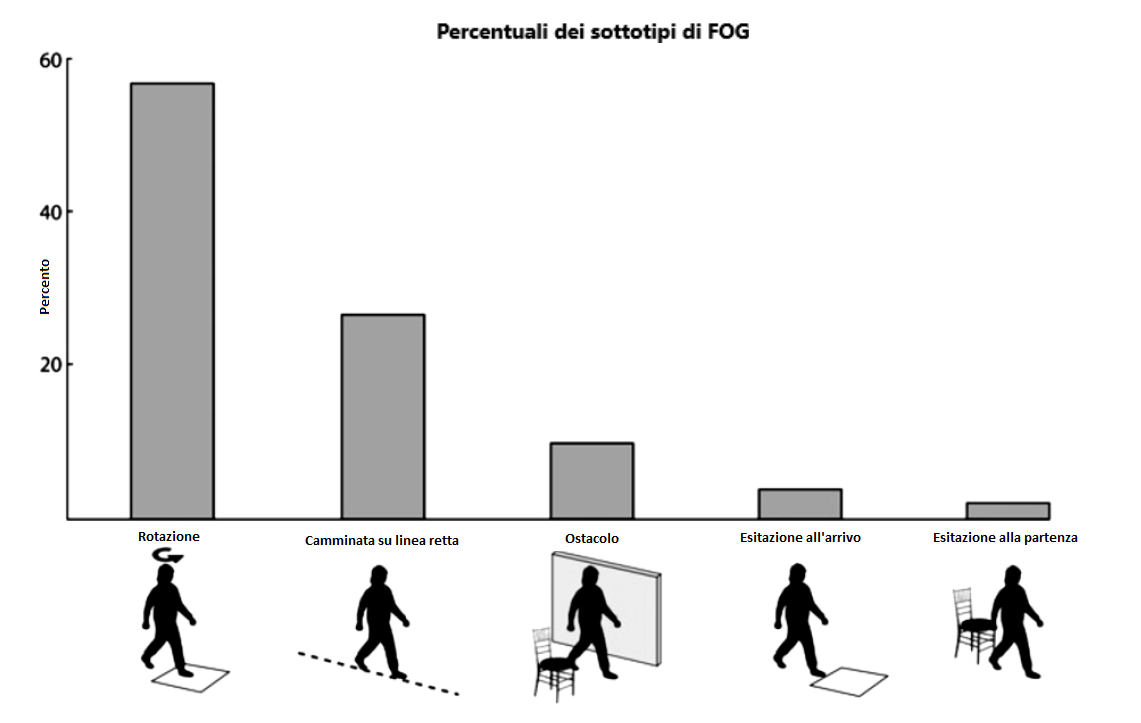
\includegraphics[scale=0.4]{images/Proportion_of_FOG_sub-types.png}
	\caption{Diversi tipi di Freezing esistenti e loro percentuale di incidenza su un certo gruppo di malati di Parkinson. [Fonte: J.M. Shine et al., 2012]}
\end{figure}
Dallo studio di Schaafsma et al.\cite{30} emerge che gli episodi di Freezing possono anche essere suddivisi in ulteriori tre sottotipi andando ad osservare i movimenti delle gambe dei pazienti e applicando la classificazione di Thompson e Marsden (1995):
\begin{enumerate}
	\item FoG associato a passi molto piccoli e strascicati con il minimo movimento in avanti (trascinamento con piccoli passi);
	\item FoG caratterizzato da tremore alle gambe, ma nessun movimento in avanti efficace (tremito da fermo);
	\item FoG caratterizzato da acinesia completa, vale a dire nessun movimento osservabile delle gambe.
\end{enumerate}
La necessità di dividere il FoG in sottogruppi dipende dal fatto che questi ultimi potrebbero avere origine differente e quindi essere provocati da cause separate.
\subsection{Influenza del FoG nella camminata}
Il Freezing of Gait influenza il pattern del cammino sia all’inizio della deambulazione sia a regime incrementando o diminuendo in modo evidente i valori dei parametri sopra riportati. Ad esempio, nei parkinsoniani che manifestano frequenti fenomeni di Freezing, la variabilità della durata del passo risulta maggiore e la lunghezza del passo minore rispetto alle situazioni in cui il Freezing è assente. Inoltre, la velocità e la lunghezza dei primi tre passi sono significativamente inferiori nei pazienti con malattia di Parkinson e con Freezing rispetto ai soggetti sani. Anche se il Freezing è tipicamente considerato un problema motorio, il fatto che spesso compaia quando il paziente si trova in spazi ristretti, suggerisce che la percezione dello spazio contribuisce in larga misura a scatenare il sintomo\cite{37}. Inoltre, i pazienti con Freezing hanno velocità media del cammino minore rispetto a pazienti sani e subiscono una riduzione ulteriore della velocità nel momento in cui si trovano a dover attraversare una porta o uno spazio stretto. Depressione e ansia possono comportare un carico cronico sulla salute mentale, e la depressione è associata con i cambiamenti di andatura, tra cui una maggiore variabilità passo-a-passo. Il Dual-Tasking, l’ansia e la depressione possono incrementare la variabilità del passo, la de-sincronizzazione di gamba destra e sinistra e l'asimmetria nei pazienti con Parkinson riducendo così la soglia per il FoG. \\

\section{Machine Learning}
Il Machine Learning (ML) è un settore dell'Intelligenza Artificiale che si occupa di studiare le modalità in cui un computer può imparare (o migliorare le sue prestazioni) dai dati\cite{10}. Un'ampia area di ricerca tratta l'apprendimento automatico di sequenze complesse di dati e compiere decisioni intelligenti su di essi. Per esempio, un tipico problema di ML è quello di programmare un computer in modo tale che possa automaticamente riconoscere codici postali scritti a mano nelle lettere, dopo aver fatto allenare il computer stesso su dei dati.
Gli algoritmi di apprendimento automatico sono tradizionalmente divisi in tre principali tipologie:
\begin{itemize}
	\item \textbf{Apprendimento supervisionato}: quando l'utente fornisce esempi (e controesempi) di quello che si deve apprendere. E' il problema più studiato	nel machine learning. Esso si pone l’obiettivo di prevedere, dato un
	elemento di cui si conoscono un insieme di parametri (features), il valore di un diverso parametro di output relativo all’elemento stesso;
	\item \textbf{Apprendimento non supervisionato}: parte da osservazioni non preclassificate;
	\item \textbf{Apprendimento con rinforzo}: tecnica di programmazione che si basa sul 	presupposto che l'algoritmo possa ricevere stimoli dall'esterno a seconda
	delle scelte fatte.
\end{itemize}
Il problema del ML è definito a partire da un universo di elementi: ciascun elemento x è descritto dai valori assunti da un insieme di features considerate come input del problema. Ad ogni x è associato un valore y di output (o target). A partire dalla conoscenza di un insieme T di elementi (denominato training set) in cui ogni elemento è descritto da una coppia ($x_i$ ,$y_i$), con $x_i$ = vettore dei valori delle d features $x_{i1}, x_{i2}, ... , x_{id}$ e $y_i$ = valore di output, si vuole derivare un modello delle relazioni sconosciute tra features e valori di output, che, dato un nuovo elemento x, consenta di predire il corrispondente valore di output y. 
\begin{figure}[]
	\centering
	\includegraphics[scale=1]{images/Tipologie_Machine_Learning.png}
	\caption{Schema delle tipologie di Machine Learning}
\end{figure}
Lo scopo dell'apprendimento supervisionato è di costruire un \textbf{modello di predizioni} basato su evidenze in presenza di incertezze. Un algoritmo di apprendimento supervisionato prende un insieme conosciuto di dati di input e di risposte ai dati (output) ed allena un modello al fine di generare predizioni ragionevoli a nuovi dati di input. Esistono due tecniche per questo approccio:
\begin{itemize}
	\item \textbf{Classificazione}: tecnica per predire risposte discrete, classificando i dati di input in categorie;
	\item \textbf{RegressionE}: tecnica per predire risposte continue.
\end{itemize}
L'apprendimento non supervisionato, invece, trova pattern nascosti o strutture intrinseche nei dati. Tale tecnica è usata per identificare inferenze da un dataset consistente di dati di input senza classi già definite. Il clustering è l'approccio più diffuso di tale tecnica ed è utilizzato per trovare gruppi nei dati.\\
L'approccio che si usa con il ML è differente da problema a problema, per cui non sempre si ha a priori un procedimento fissato da seguire, ma piuttosto si procede a tentativi ed errori, molte volte provando diverse idee ed approcci che appartengono a tale contesto. Per questo è importante definire uno schema di lavoro generale ed evidenziare alcuni punti di decisione chiave lungo il percorso:
\begin{enumerate}
	\item Accesso e caricamento dei dati: questi possono essere di tutte le forme e i tipi, incompleti o mescolati;
	\item Pre-processamento dei dati: applicazione di filtri o ri-campionamento;
	\item Derivazione di feature:trovare caratteristiche peculiari a partire dai dati;
	\item Allenamento del modello di ML: può essere un procedimento lungo, poichè dipende da molti parametri;
	\item Integrazione del modello in un sistema di produzione.
\end{enumerate}
\begin{figure}[]
	\centering
	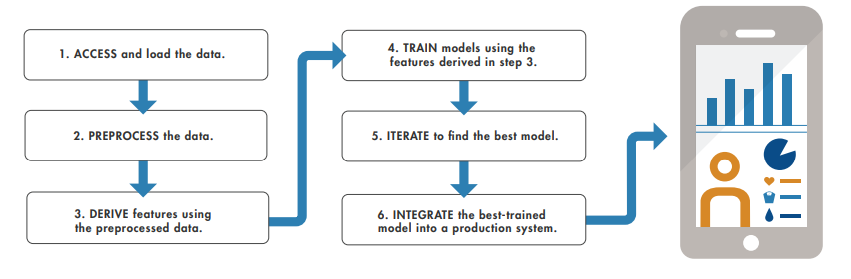
\includegraphics[scale=0.55]{images/Workflow_ML.png}
	\caption{Esempio di Workflow tramite Machine Learning}
\end{figure}
La scelta della modalità supervised o unsupervised si basa sui vantaggi e svantaggi di entrambe: la modalità supervised riesce a predire la giusta classe per le istanze appartenti al test set ma richiede una consistente quantità di istanze annotate e questo può rappresentare un processo costoso se effettuato manualmente. La modalità unsupervised tipica del clustering, invece, ha il vantaggio di non richiedere un training già annotato (situazione particolarmente frequente quando si
ricorre al ML) ma fa più fatica ad etichettare correttamente i dati ed ottiene una precisione più scarsa rispetto al metodo supervisionato nell'associare le istanze ai cluster corretti. 

\subsection{Analisi dei Gruppi}
Con il termine Cluster Analysis, o analisi dei gruppi, si intendono le procedure che permettono di individuare, all'interno di un insieme di oggetti di qualsiasi natura, alcuni sottoinsiemi, \textbf{clusters} appunto, mutuamente esclusivi e tendenzialmente omogenei al loro interno. Le tecniche di Cluster Analysis creano i gruppi in modo tale che ogni osservazione sia molto simile a tutte le altre che appartengono allo stesso gruppo, in funzione di alcuni criteri prestabiliti. Alla fine del procedimento, i cluster finali dovrebbero esibire un'alta omogeneità interna (intra-cluster) ed un'alta eterogeneità esterna (inter-cluster), quindi gli oggetti all'interno dei cluster saranno vicini tra loro, mentre gli oggetti che appartengono a differenti cluster saranno più lontani tra loro.\\
L'analisi dei gruppi rientra tra le tecniche di tipo esplorativo e pertanto non è necessaria alcuna assunzione a priori, anche se impone una serie di decisioni durante l'analisi:
\begin{itemize}
	\item Scelta delle variabili;
	\item Criteri di similarità o distanza;
	\item Tecniche di aggregazione;
	\item Numero dei gruppi da ottenere;
	\item Valutazione della qualità della soluzione;
	\item Scelta fra le diverse possibili soluzioni.
\end{itemize}
\begin{figure}[]
	\centering
	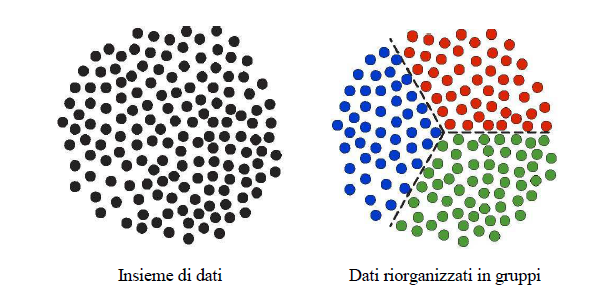
\includegraphics[scale=0.8]{images/Esempio_Cluster.png}
	\caption{Rappresentazione dei dati e dei gruppi ottenuti con l'analisi dei gruppi}
\end{figure}
Per classificare e raggruppare gli elementi in gruppi omogenei, è necessario introdurre il concetto di prossimità o similarità. Due individui sono vicini quando la loro similarità o distanza è piccola o, equivalentemente, quando la loro similarità è grande.
% Le principali misure di similarità sono illustrate in tabella \ref{TAB:SIMILARITA'}.

%\begin{table}[h!]
%	\begin{tabular}{| l | c | c | }
%	\multicolumn{1}{|l|}{Tipo di dato} &  
%	\multicolumn{1}{c|}{Misura} &
%	\multicolumn{1}{c|}{Formula}\\
%	\hline
%	\hline
%	Binario					&	Coefficiente di Sokal		&	$S_{ij}=(a+d)/(a+b+c+d)$	\\
%	Binario					&	Coefficiente di Jaccard		& 	$S_{ij}=a/(a+b+c)$\\
%	Categorici non binari	& 	Media delle variabili		&	$S_{ij}=(1/p) \sum_{k=1}^{p} s_{ijk}$\\
%	Dati Continui			& 	Distanza Euclidea			&	$d_{ij}=[\sum_{k=1}^{p}(x_{ik}-x_{jk})^2]^{1/2}$\\
%	Dati Continui			& 	Distanza City Block			&	$d_{ij}=\sum_{k=1}^{p}|x_{ik}-x_{jk}|$\\
%	
%\end{tabular}
%\vspace{0.1cm}
%\caption{Misure di Similarità}
%%\vspace{-0.2cm}
%\label{TAB:SIMILARITA'}
%\end{table}

I principali algoritmi di clustering sono descritti nelle prossime sottosezioni.
\subsubsection{K-Means}
Il K-Means è un algoritmo di clustering partizionale che permette di suddividere un insieme di oggetti in K gruppi sulla base dei loro attributi. E' una variante dell'algoritmo di aspettativa-massimizzazione(EM) il cui obiettivo è determinare i K gruppi di dati generati da distribuzioni gaussiane. Si assume che gli attributi degli oggetti possano essere rappresentati come vettori e che quindi formino uno spazio vettoriale. L'obiettivo che l'algoritmo si prepone è di minimizzare la varianza intra-cluster, dove ogni cluster viene identificato mediante un centroide o punto medio. L'algoritmo segue una procedura iterativa:
\begin{enumerate}
	\item Sceglie in modo casuale o euristico k punti che rappresentano i centroidi iniziali dei cluster;
	\item Ripete fino a che gli assegnamenti non cambiano
	\subitem Assegna ciascun oggetto al cluster più vicino, ossia il cui centro risulta il più vicino all'oggetto dato
	\subitem Calcola i centroidi dei cluster.
\end{enumerate}
L'algoritmo converge molto velocemente, infatti è stato osservato che il numero di iterazioni è minore del numero di punti da osservare. In termini di qualità delle soluzioni, però, l'algoritmo non garantisce il raggiungimento dell'ottimo globale poiché la soluzione dipende largamente dal set di cluster iniziale. Un rimedio a questo aspetto è applicare l'algoritmo più volte e, fra tutte le soluzioni prodotte, scegliere quella più soddisfacente. Un altro svantaggio è che l'algoritmo richiede di scegliere a priori il numero di cluster da trovare, per cui se i dati non sono naturalmente partizionati si ottengono risultati strani. Inoltre, l'algoritmo funziona bene solo quando sono individuabili cluster sferici nei dati.
\begin{figure}[h!]
	\centering
	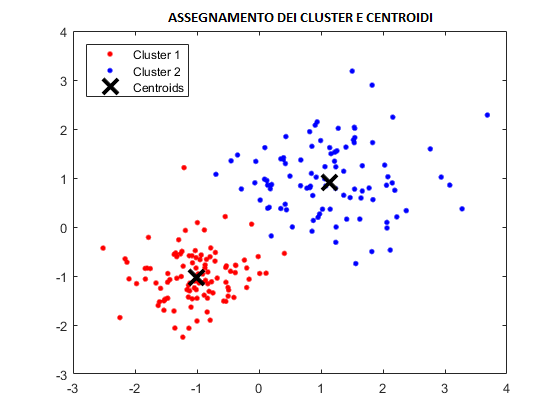
\includegraphics[scale=0.50]{images/example_kmeans.png}
	\caption{Esempio di assegnazione dei dati tramite l'algoritmo k-means}
\end{figure}
\subsubsection{K-Medoids}
K-medoids è un algoritmo di clustering partizionale correlato all'algoritmo K-means. Prevede in input un insieme di n oggetti e un numero k che determina quanti cluster si vogliono in output. Entrambi gli algoritmi sono partizionali (suddividendo il dataset in gruppi) ed entrambi cercano di minimizzare l'errore quadratico medio, la distanza tra punti di un cluster e il punto designato per esserne il centro. In K-means il punto è artificiale, dato che è la pura media di tutti i punti nel cluster. Nel K-medoids è usato il punto collocato più centralmente, in questo modo il centro è uno dei datapoint attuali. K-medoids è più robusto al rumore e agli outlier rispetto al k-means. Un medoid può essere definito come un oggetto di un cluster la cui dissimilarità media rispetto a tutti gli oggetti nel cluster è minima, in questo modo esso sarà il punto più centrale di un dato dataset.
L'algoritmo di clustering è il seguente:
\begin{enumerate}
	\item Si scelgono arbitrariamente k oggetti (dove K è il numero di cluster che si vogliono ottenere) come punti medoid da un insieme di n data point (n>k);
	\item In seguito alla selezione di k punti medoid, si associa ogni oggetto nel dato dataset al più simile medoid. La similarità è definita usando misure di distanza;
	\item Si seleziona in modo casuale un oggetto non medoid O';
	\item Si calcola il costo totale S per lo scambio del medoid iniziale nell'oggetto O';
	\item Se S<0, allora si scambia il medoid iniziale con il nuovo (se S<0 allora ci sarà un nuovo insieme di medoid);
	\item Si ripetono i passi dal 2 al 5 sino a quando si hanno cambiamenti nel medoid.
\end{enumerate}
\begin{figure}[h!]
	\centering
	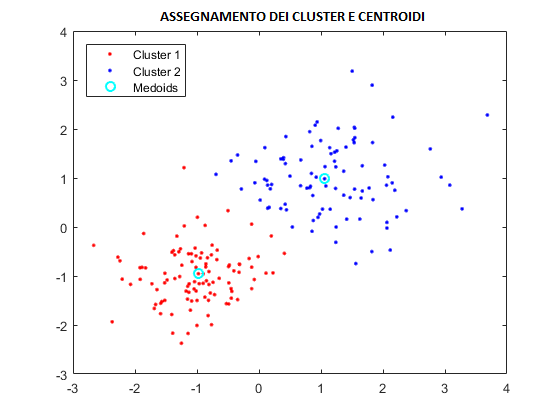
\includegraphics[scale=0.50]{images/example_kmedoids.png}
	\caption{Esempio di assegnazione dei dati tramite l'algoritmo k-medoids}
\end{figure}
\subsubsection{Hierarchical}
Il clustering gerarchico è un approccio di clustering che mira a costruire una gerarchia di cluster. Le strategie per il clustering gerarchico sono tipicamente di due tipi:
\begin{itemize}
	\item Agglomerativo: si tratta di un approccio "bottom up" (dal basso verso l'alto) in cui si parte dall'inserimento di ciascun elemento in un cluster differente e si procede quindi all'accorpamento graduale di cluster a due a due;
	\item Divisivo: si tratta di un approccio "top down" (dall'alto verso il basso) in cui tutti gli elementi si trovano inizialmente in un singolo cluster che viene via via suddiviso ricorsivamente in sotto-cluster.
\end{itemize}
Il risultato di un clustering gerarchico è rappresentato in un dendrogramma. Questo è uno strumento grafico per la visualizzazione del coefficiente di similarità quantificato dalle varie macchine e dai vari cluster nel processo di “raggruppamento”. Il dendrogramma viene utilizzato per fornire una rappresentazione grafica del processo di raggruppamento delle istanze che esprime nell'asse delle ascisse la distanza logica dei clusters secondo la metrica definita, nell'asse delle ordinate il livello gerarchico di aggregazione (valori interi positivi). 
La scelta del livello gerarchico (del valore dell'asse Y) definisce la partizione rappresentativa del processo di aggregazione.\\
Per decidere quali cluster devono essere combinati (approccio agglomerativo) o quale cluster deve essere suddiviso (approccio divisivo) è necessario definire una misura di dissimilarità tra cluster. Nella maggior parte dei metodi di clustering gerarchico si fa uso di metriche specifiche che quantificano la distanza tra coppie di elementi e di un criterio di collegamento che specifica la dissimilarità di due insiemi di elementi (cluster) come funzione della distanza a coppie tra elementi nei due insiemi. Le metriche di distanza più comuni sono: euclidea, Manhattan, uniforme, Mahalanobis, Hamming. Le metriche più diffuse sono: complete linkage (massima distanza tra due punti), single linkage (minima distanza tra due punti) o average linkage (media distanza tra due punti).
\begin{figure}[h!]
	\centering
	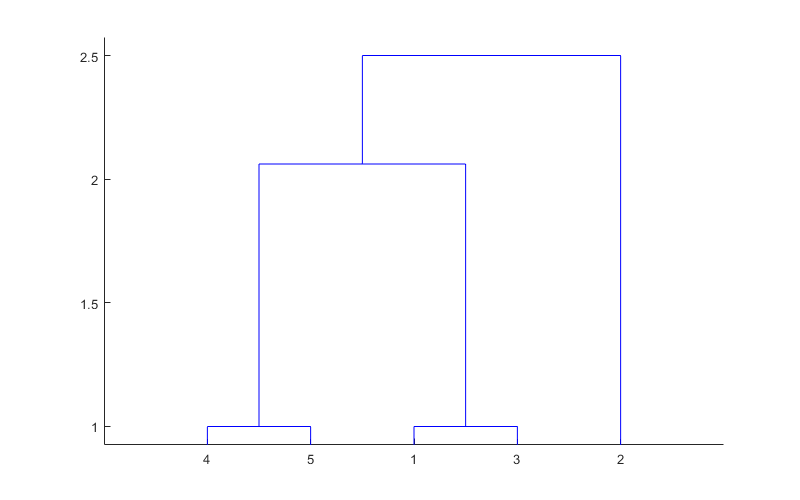
\includegraphics[scale=0.50]{images/example_dendogram.png}
	\caption{Esempio di assegnazione dei dati tramite cluster gerarchico e la sua rappresentazione tramite dendogramma}
\end{figure}
\subsubsection{Reti Neurali}
Una Rete Neurale é un modello matematico che calcola la funzione output=f(input,pesi) al variare dei pesi e senza specificare la forma della funzione f, o anche un sistema dinamico avente la topologia di un grafo orientato con nodi, i neuroni artificiali, ed archi, i pesi sinaptici, nel quale il termine rete è riferito alla topologia dei collegamenti tra i neuroni. Le self-organizing map (SOM) sono una tipologia di reti neurali artificiali. È addestrata usando l'apprendimento non supervisionato per produrre una rappresentazione dei campioni di training in uno spazio a bassa dimensione preservando le proprietà topologiche dello spazio degli ingressi. Questa proprietà rende le SOM particolarmente utili per la visualizzazione di dati di dimensione elevata. Le SOM sono reti neurali a connessioni laterali dove i neuroni di uscita sono organizzati in griglie di bassa dimensione (generalmente 2D o 3D). Ogni ingresso è connesso a tutti i neuroni di uscita. Ad ogni neurone è associato un vettore dei pesi della stessa dimensione dei vettori d'ingresso. La dimensione del vettore d'ingresso è generalmente molto più alta della dimensione della griglia di uscita. L'obiettivo dell'apprendimento nelle SOM è di specializzare parti differenti del reticolo SOM a rispondere similmente a particolari pattern d'ingresso.\\
L'algoritmo di clustering è il seguente:
\begin{enumerate}
	\item Assegna ai vettori dei pesi valori casuali;
	\item Prende un vettore d'ingresso;
	\item Attraversa ogni nodo della mappa ed usa la distanza euclidea per trovare somiglianze fra il vettore d'ingresso ed il vettore dei pesi di ogni singolo nodo della mappa, individuando il nodo a distanza minore (questo nodo verrà chiamato Best Matching Unit o BMU);
	\item Aggiorna i nodi del vicinato di BMU "tirandoli" più vicino al vettore d'ingresso.
\end{enumerate}
Ci sono due modi per interpretare una SOM:
\begin{itemize}
	\item Dato che nella fase di addestramento i pesi di tutto il vicinato sono spostati nella stessa direzione, elementi simili tendono ad eccitare neuroni adiacenti. Perciò le SOM formano una mappa semantica dove campioni simili vengono mappati vicini e dissimili distanti;
	\item Un altro modo di considerare i pesi neuronali è di pensarli come punti distribuiti nello spazio degli ingressi. Questi formano un'approssimazione della distribuzione dei campioni d'ingresso. Più neuroni puntano a regioni con un'elevata concentrazione di campioni di addestramento, e meno in zone dove i campioni sono scarsi.
\end{itemize}
\begin{figure}[h!]
	\centering
	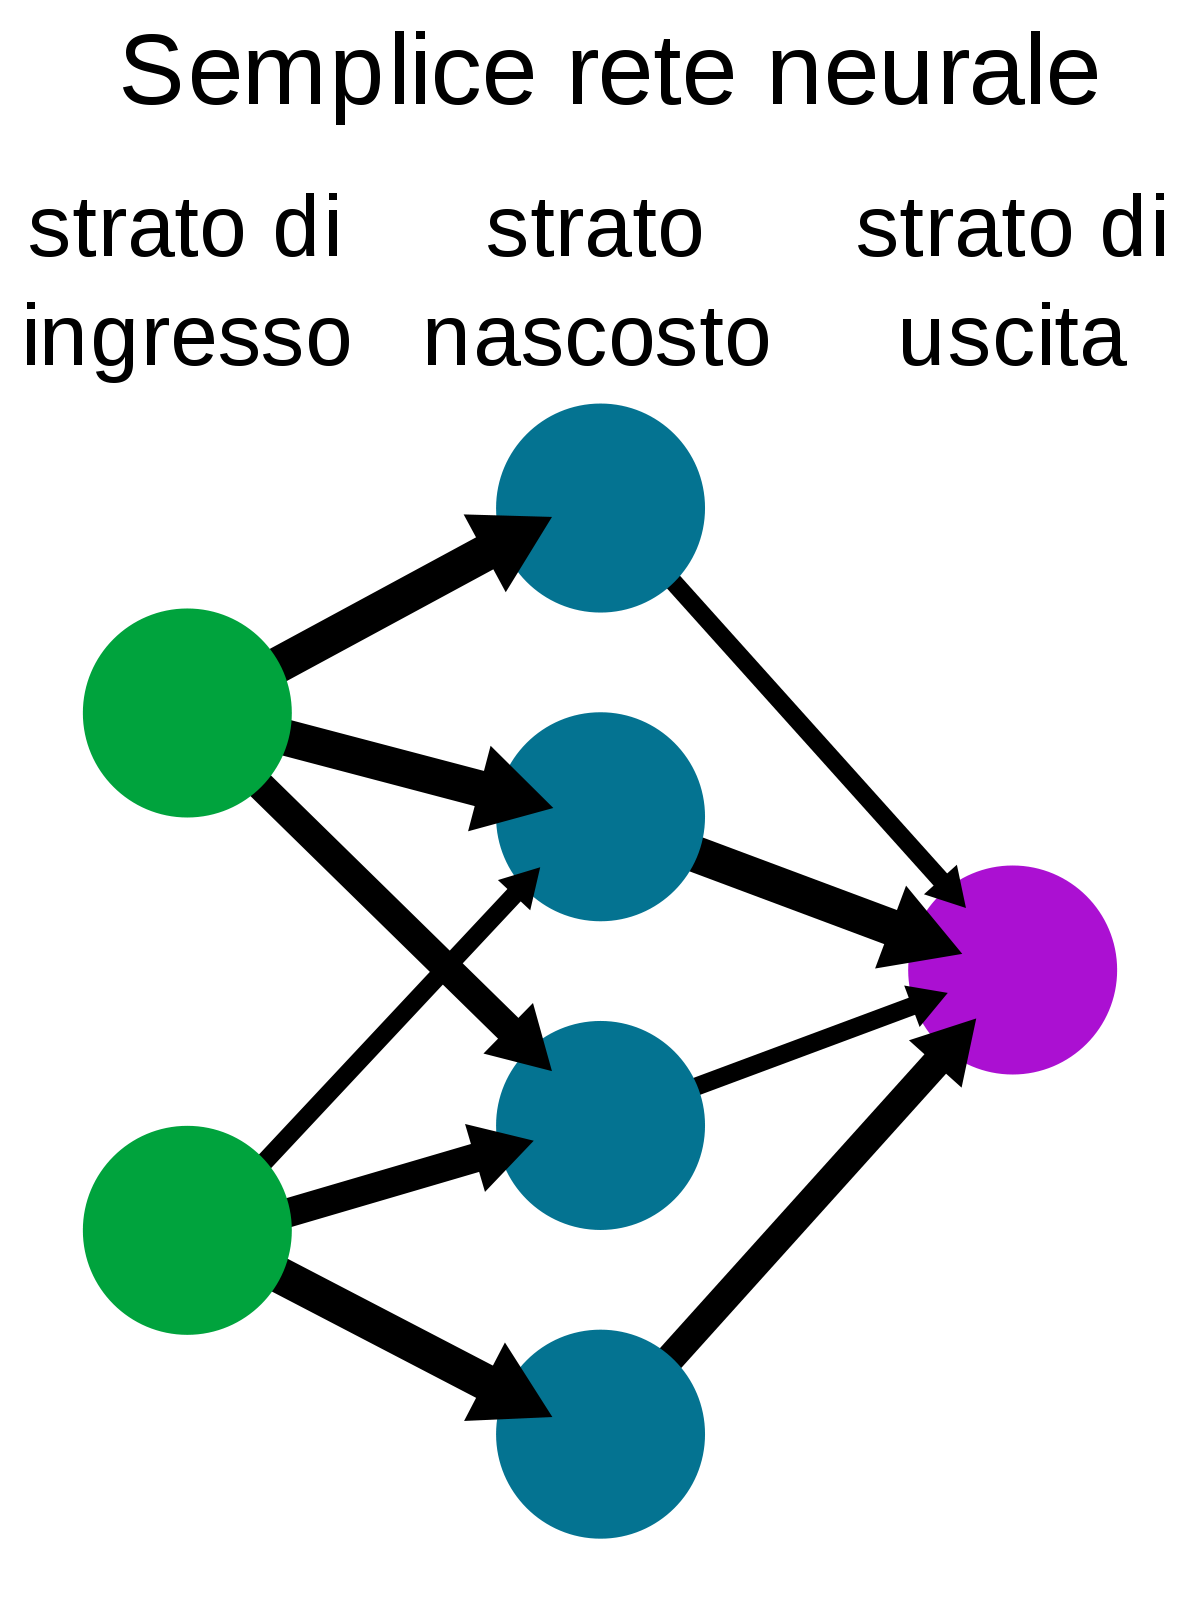
\includegraphics[scale=0.50]{images/example_som.png}
	\caption{Schema input-output per una SOM}
\end{figure}
\subsubsection{Fuzzy C-Means}
Il Fuzzy C-means (anche riferito come soft clustering) è un algoritmo di clustering nel quale ogni punto può appartenere a più di un cluster. L'algoritmo è molto simile al k-means, ma in questo contesto viene assegnato ad ogni punto un grado di appartenenza. Questo indica il grado con cui un determinato punto appartiene ad un certo cluster. L'algoritmo di clustering è il seguente:
\begin{enumerate}
	\item Sceglie un numero K di cluster;
	\item Assegna randomicamente dei coefficienti di appartenenza ad un cluster per ogni punto;
	\item Calcola il centroide di ogni cluster;
	\item Per ogni punto, calcola il suo grado di appartenenza ai clusters;
	\item Itera fino ad avere convergenza.
\end{enumerate}

\begin{figure}[]
	\centering
	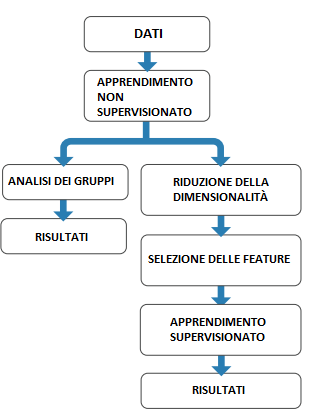
\includegraphics[scale=0.8]{images/Approcci_Clustering.png}
	\caption{Rappresentazione dei possibili approcci usando strategie di clustering}
\end{figure}
\subsection{Classificazione}
I principali approcci di classificazione sono due. In un modello parametrico, il modello stesso è preventivamente caratterizzato da un vettore X di parametri: si suppone quindi che esista una relazione tra features e input e che tale relazione sia rappresentabile all’interno di una famiglia di
relazioni parametriche rispetto a X che costituisce un modello; in altre parole, un'assegnazione di valori al vettore X definisce una specifica relazione della famiglia. Gli elementi nel training set sono utilizzati proprio per derivare tale
assegnazione di valori ai parametri (o una distribuzione di probabilità per tali valori), dopo di che non sono più utilizzati. In un modello non parametrico, invece, il numero di parametri cresce con la dimensione del training set: sostanzialmente, ogni singola previsione, in questo caso, richiede l’utilizzo dell’intero training set. Un esempio di approccio non parametrico sono i classificatori di tipo nearest neighboor, in cui si determina l'elemento $x_i$ del training set più vicino a x e si impone il valore della nuova previsione y associata a x uguale al valore $y_i$ dell’elemento $x_i$.\\
I principali algoritmi di classificazione sono:
\begin{itemize}
	\item \textbf{Decisione Tree}: si tratta di un classificatore con struttura ad albero, in cui ogni nodo può essere o foglia o nodo interno: se foglia, indica il valore della classe assegnata all'istanza; se nodo interno, specifica il test effettuato su un attributo. Per ciascun valore assunto da un attributo in un test, l'algoritmo crea un ramo ed il relativo sottoalbero. Il focus principale dell'algoritmo di crescita del decision tree è il come scegliere gli attributi da testare in ciascun nodo interno dell'albero. L'obiettivo è selezionare gli attributi più utili per classificare le istanze di training
	attraverso una strategia top down, che consiste in una ricerca greedy degli
	attributi senza tornare a riconsiderare le precedenti scelte. Il criterio di split (suddivisione) con cui crea un nuovo nodo si basa sul massimo guadagno di informazione (info gain). In pratica sceglie l'attributo che riesce a dividere “meglio” le istanze appartenenti a classi diverse (detto anche criterio di massima riduzione di incertezza). Quando tutti gli elementi in un nodo hanno la medesima classe, l'algoritmo non procede con ulteriore split (criterio di stopping).
	\item \textbf{K-Nearest-Neighbors}: esso memorizza le istanza del training, poi, basandosi su un criterio di vicinanza, mette in relazione l'istanza da classificare con alcune istanze del training set presenti nello spazio delle feature.  In pratica, l'istanza è classificata “a maggioranza” in base alla
	classe più comune tra le k istanze più vicine del training. Tutto il lavoro è fatto dal classificatore in runtime. Data una nuova istanza x da classificare, il classificatore cerca i k esempi del training che sono più “simili” a x e
	guarda le loro etichette. Qualsiasi label ricorra più frequentemente tra le k label più vicine è scelta per assegnare la classe a x.
	\item \textbf{Support Vector Machine}:  l'idea principale di questo classificatore consiste nel rappresentare gli esempi del training come punti nello spazio mappati in modo tale che punti appartenenti a classi differenti siano separati dal più ampio gap possibile. I punti che mappano il test set saranno assegnati ad una categoria o all'altra in base al lato del gap su cui cadono. Più specificatamente, SVM costruisce un iperpiano ed esegue una buona separazione quando l'iperpiano ha la più ampia distanza dai punti di training più vicini di ciascuna classe. Ci sono molti iperpiani che potrebbero classificare il dato. La miglior scelta è quella di selezionare l'iperpiano che rappresenta la più ampia separazione, o margine, tra due classi, ossia l'iperpiano tale che la distanza tra esso e il punto più vicino su ciascun lato sia massima.
\end{itemize}
\subsection{Validazione della Classificazione}
Al fine di valutare la bontà della classificazione effettuata, viene introdotto il concetto di \textbf{Matrice di Confusione}. Essa è una matrice nxn, con n=numero di classi, nella quale vengono messe a confronto le etichette reali con quelle del classificatore proposto. La figura \ref{immagine_matrice_confusione_2classi}  rapprestra la matrice di confusione con 2 classi possibili:
\begin{itemize}
	\item Il \textbf{Vero Positivo} indica quante volte ho classificato giusto l'etichetta che io considero come positiva, ad esempio la classe 1;
	\item Il \textbf{Vero Negativo} indica quante volte ho classificato giusto l'etichetta che io considero come negativa, ad esempio la classe 2;
	\item Il \textbf{Falso Positivo} indica quante volte ho classificato sbagliato l'etichetta che io considero come positiva, ossia il mio classificatore ha etichettato il mio campione con la classe 1, ma in realtà quella misurazione appartiene alla classe 2;
	\item Il \textbf{Falso Negativo} indica quante volte ho classificato sbagliato l'etichetta che io considero come negativa, ossia il mio classificatore ha etichettato il mio campione con la classe 2, ma in realtà quella misurazione appartiene alla classe 1;
\end{itemize}
\begin{figure}[h!]
	\centering
	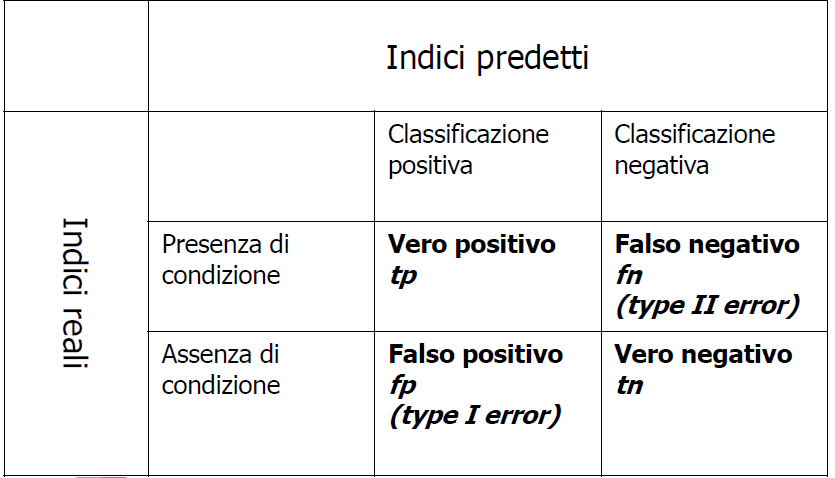
\includegraphics[scale=0.5]{images/matrice_confusione.png}
	\caption{Rappresentazione della matrice di confusione per 2 classi}
	\label{immagine_matrice_confusione_2classi}
\end{figure}
La condizione ideale di classificazione sarebbe quella in cui la matrice di confusione è diagonale, ossia non presento falsi positivi o falsi negativi. Da questa si possono ricavare varie misure, tutte nell'intervallo [0,1]:
\begin{itemize}
	\item \textbf{Accuratezza}: $\dfrac{tp+tn}{tp+tn+fp+fn}$
	\item \textbf{Precisione}: $\dfrac{tp}{tp+fp}$
	\item \textbf{Sensitività}: $\dfrac{tp}{tp+tn}$
	\item \textbf{F1-measure}: $\dfrac{2*precisione*sensitivita' }{sensitivita' + precisione}$
	\item \textbf{Specificità}: $\dfrac{tn}{fp+tn}$
\end{itemize}
Nel caso di più classi, si possono generalizzare le misure di precisione e sensitività associate alle singole classe, mentre il concetto di accuratezza resta sempre lo stesso. La figura \ref{immagine_matrice_confusione_cclassi} rappresenta la generalizzazione delle formula suddette.
\begin{figure}[h!]
	\centering
	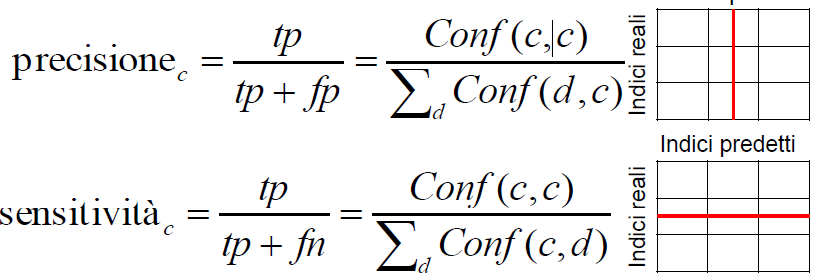
\includegraphics[scale=0.5]{images/matrice_confusione_cclassi.png}
	\caption{Rappresentazione della matrice di confusione per c classi}
	\label{immagine_matrice_confusione_cclassi}
\end{figure}

\section{Riduzione della dimensionalità}
\subsection{Analisi Delle Componenti Principali}
\begin{figure}[]
	\centering
	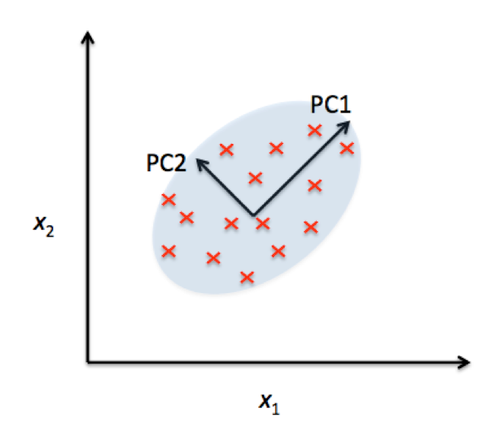
\includegraphics[scale=0.8]{images/pca.png}
	\caption{Rappresentazione del cambio di dimensionalità tramite PCA}
\end{figure}
L'analisi in componenti principali o \textbf{PCA} è una tecnica per la semplificazione dei dati, con lo scopo primario di ridurre un numero più o meno elevato di variabili in alcune caratteristiche latenti. Questo procedimento prende il nome di \textbf{feature reduction}. Ciò avviene tramite una trasformazione lineare delle variabili che proietta quelle originarie in un nuovo sistema cartesiano nel quale la nuova variabile con la maggiore varianza viene proiettata sul primo asse, la seconda variabile per dimensione della varianza sul secondo asse e così via. La riduzione della complessità avviene quindi limitandosi ad analizzare le principali (per varianza) tra le nuove variabili. Diversamente da altre trasformazioni lineari, in questa tecnica sono i dati stessi che determinano i vettori di trasformazione.\\
Un metodo per calcolare la componente $w_i$ (ossia quella che effettua la trasformazione per la variabile i) utilizza la \textbf{matrice delle covarianze} di x, mentre un altro metodo possibile usa la matrice dei coefficienti di correlazione. Innanzitutto, si devono trovare gli autovalori della matrice di covarianza: Si ottengono così tanti autovalori quante sono le variabili x. L'autovalore con il maggiore valore corrisponde alla dimensione w che ha la maggior varianza: esso sarà dunque la varianza della componente principale numero 1. Per ciascun autovalore viene calcolato il corrispondente autovettore , ossia la matrice dei coefficienti che moltiplicano le vecchie variabili x nella combinazione lineare per l'ottenimento delle nuove variabili w. La matrice degli autovettori viene definita anche matrice di rotazione V e, eseguendo l'operazione $W = V*X $, dove W è il vettore colonna avente come elementi le nuove variabili $w_1,w_2,..$ e X è il vettore colonna avente come elementi le vecchie variabili $x_1,x_2,..$, si possono trovare le coordinate di ciascun punto nel nuovo spazio vettoriale. Alla fine, quindi, si tengono solo le componenti le quali, sommate tra di loro, esprimono una certa varianza (es. 90\% della varianza dei dati), mentre le altre vengono ignorate. In questo modo, partendo da n variabili iniziali, posso arrivare a (n-k) nuove variabili, dove k è il numero di componenti che non mi servono per raggiungere la soglia di varianza prefissata. Un'altrà possibilità è invece quella di scegliere a priori la quantità (n-k) di nuove variabili da tenere, ossia quante feature voglio avere dopo la trasformazione.
\subsection{Analisi dei Discriminanti Lineari}\label{Fisher}
Mentre la PCA è utile per la rappresentazione dei pattern (es. riconoscimento di immagini), l'analisi dei discriminanti lineari o \textbf{LDA} viene usata per discriminare tali pattern, ossia per trovare delle misure che mi permettano di dividere in più classi i miei dati. Entrambe vengono usate per la riduzione della dimensionalità delle variabili di input.\\
L'obiettivo della LDA è quello di trovare un vettore w, di trasformazione, tale per cui classi differenti siano ben separate, mentre la diffusione di ogni classe sia ridotta il più possibile. In pratica, si tratta di trovare una soluzione al cosidetto criterio di Fisher: \begin{equation} J_F = \dfrac{w^TS_Bw}{w^TS_ww}  \end{equation} nella quale $S_B$ ed $S_W$ sono rispettivamente la matrice di dispersione tra le classi e la matrice di dispersione all'interno della classe. Nel caso di due classi, la $S_B$ si calcola come: \begin{equation} S_B = (m_1 - m_2)(m_1 - m_2)^T \end{equation} dove $m_1$ rappresenta la media della classe 1 e $m_2$ quella della classe 2. $S_w$, invece, si calcola come \begin{equation}S_W = \sum_{i=1}^{c} \sum_{x \in w_i}^{} (x - m_i)(x-m_i)^T\end{equation} con $m_i$ = media della classe i e c = numero di classi.\\
La soluzione del criterio di Fisher viene chiamata anche \textbf{Problema dell'Autovalore Generalizzato} e viene rappresentata da tale equazione: \begin{equation}S_Bw=\lambda S_ww\end{equation} e, se $S_w$ è invertibile, diventa \begin{equation}S_w^{-1}S_Bw=\lambda w\end{equation} corrispondente al problema degli autovalori regolari che coinvolge $S_W^{-1}S_B$. Una volta che w viene trovato, le feature cercate vengono calcolate: \begin{equation}y = w^Tx\end{equation} le quali possono essere usate per allenare l'algoritmo di classificazione scelto e procedere alla predizione su nuovi dati.\\
Nel caso si abbiano più di 2 classi, la matrice di dispersione tra le classi, la quali misura la separazione tra le classi, diventa: \begin{equation}S_B=\sum_{i=1}^{c} n_i(m_i-m)(m_i-m)^T\end{equation} con $n_i$ = numero di campioni di training appartenenti alla classe i ed m = media di tutti i campioni di training. Ci saranno quindi C-1 autovettori, ognuno proveniente da una soluzione di (3.5), che potrebbero non essere ortogonali tra loro ma formano uno sottospazio lineare tale per cui il criterio di Fisher è massimizzato. Questi vengono inseriti in una matrice W e si calcolano le feature come in (3.6). 
\begin{figure}[]
	\centering
	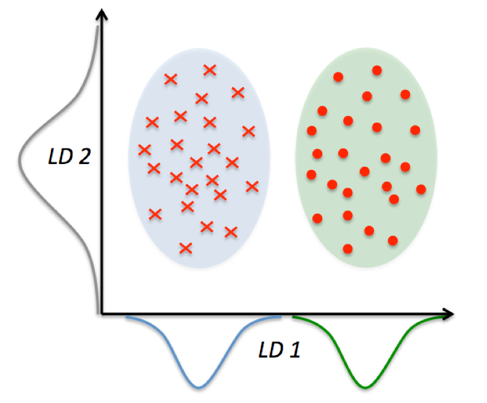
\includegraphics[scale=0.8]{images/lda.png}
	\caption{Rappresentazione del cambio di dimensionalità tramite LDA}
\end{figure}